\documentclass[../main.tex]{subfiles}
\begin{document}
	\newpage
	\subsection{Sprint 4}
	
	\par Beim 4. Sprint wurden Verbesserungen am Spiel-Kreislauf vorgenommen
	
	\begin{itemize}
		\item Task vom vorherigen Sprint
		\begin{itemize}
			\item Definiere Farbschema für das Spiel [2]
		\end{itemize}
	
		\item Bugs
		\begin{itemize}
			\item Tilestack erhält keine neuen Tiles wenn der Score steigt [2]
			\item Benutzer kann Tiles durch die UI platzieren [3]
			\item Benutzer kann die Kamera zoomen wenn das Spiel pausiert ist [2]
			\item Untere drittel des Spielfelds wird nicht richtig angezeigt [3]
			\item Es wird nicht das erste Tile aus dem Stack in die Hand genommen [2]
		\end{itemize}
	
		\item Fachbericht schreiben
		\begin{itemize}
			\item Entwurf Fachbericht schreiben [8]
		\end{itemize}
	
		\item Hand soll Behavior/Nature anzeigen
		\begin{itemize}
			\item Auf der Hand\improvement{Hand} soll die Nature und das Behavior sichtbar sein [8]
		\end{itemize}
	
		\item Tiles sollen drehbar sein
		\begin{itemize}
			\item Definiere Knöpfe um Tiles zu drehen [2]
			\item Behavior erweitern um mit der Drehung zu funktionieren [5]
			\item Leuchten der Tiles soll mit der Drehung funktionieren [2]
		\end{itemize}
	
		\item Wahrscheinlichkeiten für Tilekombinationen anpassen
		\begin{itemize}
			\item Komponente von Tiles sollen Gewichte erhalten [1]
			\item Wahrscheinlichkeit für Tiles mit Gewichte berechnen [5]
			\item Tilestack soll entsprechend den Wahrscheinlichkeiten neue Tiles generieren [1]
		\end{itemize}
		
		\item Verschiedene Animationen für Tiles erstellen
		\begin{itemize}
			\item Animation erstellen für entfernen eines Tiles [5]
			\item Animation erstellen für die Materialänderung [2]
			\item Animation hinzufügen für das platzieren von Tiles [2]
		\end{itemize}

		\item Spiel soll enden, wenn keine Tiles mehr platziert werden können
		\begin{itemize}
			\item Game Over Ansicht mit Score anzeigen [3]
			\item Game Over Ansicht soll Neustart sowie zurück zum Menü erlauben [2]
			\item Game Over Ansicht soll keine Feldmanipulationen erlauben [1]
		\end{itemize}
	\end{itemize} 

	\par Die vom vorherigen Sprint übernommene Task \emph{Definiere Farbschema für das Spiel} wurde diesen Sprint beendet. Es wurde sich für eine Farbkombination entschieden, die auch für Personen mit Sehschwächen bedienbar ist. Die Tasks \emph{Animation erstellen für das entfernen eines Tiles} sowie \emph{Animation erstellen für die Materialänderung} wurden nicht abgeschlossen und werden für den Moment auch nicht mehr berücksichtigt. Der Aufbau von den Tiles erlaubt im Moment nicht die Implementierung dieser beiden Animation und würde einen grösseren Refactor mit sich bringen. Da dies aber nur visuelle Verbesserungen sind und nicht Prioritär für den MVP, werden sie momentan beiseite geschoben. Die restlichen Tasks wurden alle erfolgreich erledigt.
	
	\begin{figure}[H]
		\centering
		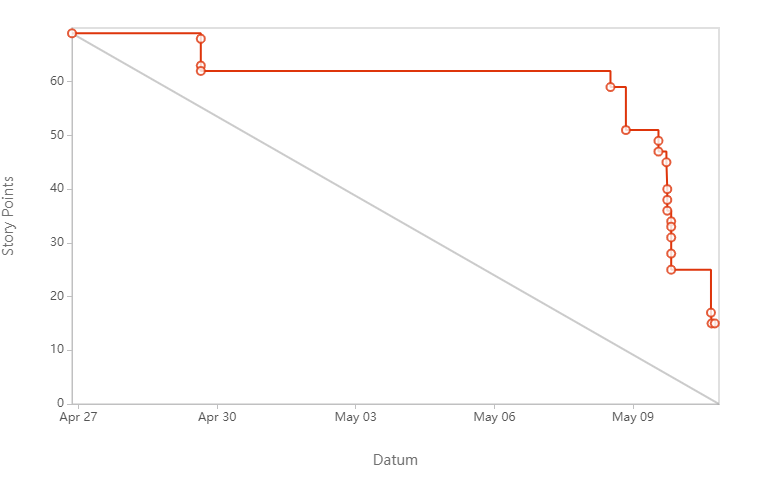
\includegraphics[width=0.5\textwidth]{Sprint_4_Burndown_Chart}
		\caption{Sprint 4 Burndown-Chart}
	\end{figure}



\end{document}